\textnormal{ 
\begin{itemize}
\item We performed data cleaning and preprocessing steps to prepare a CSV to be used in the analysis.
\begin{itemize}
\item Check for nulls (no null values in any column)
\item Calculate conversion rates from each currency to USD and prepare a new column of payments in US Dollars
\item Create a unique id by hashing bank + '\_' + account
\item Convert timestamp columns into integer year, month, day, hour, minute columns to save space
\item Output a 'clean' CSV for use in visualizations and modeling
\end{itemize}
\item We use the clean data to create two CSVs with the account data (accounts.csv) and the transaction data (transactions.csv)
\item We import these account and transaction information data into Neo4j and build a database.
\item We build a web application that primarily uses client-server architecture with MVT (Model, View, Template) design pattern. 
\begin{figure}[htp]
    \centering
    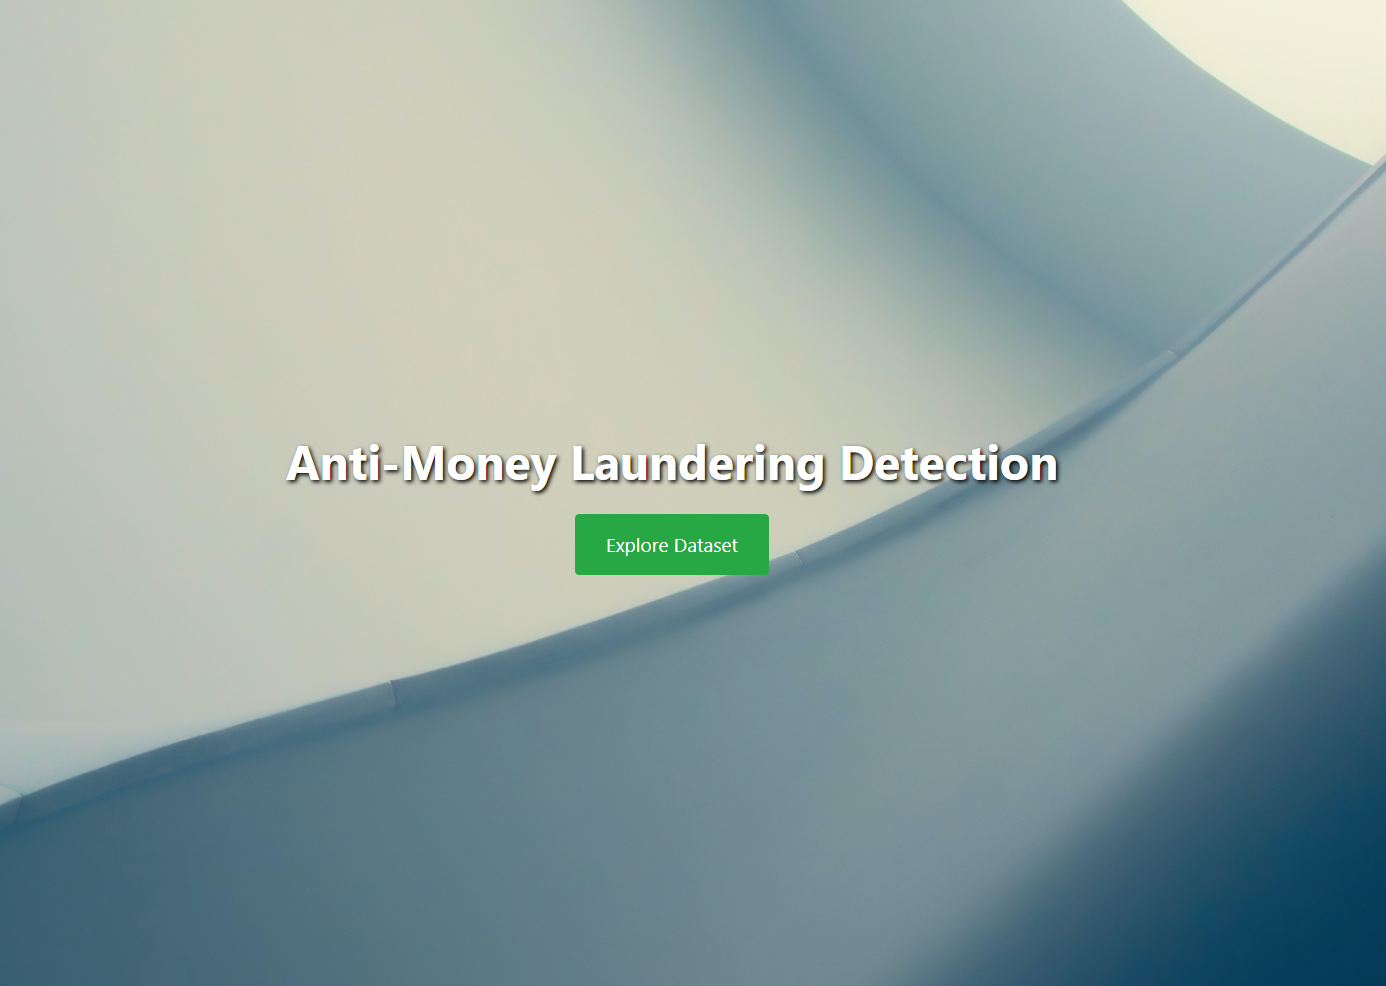
\includegraphics[width=6cm]{imgs/home.png}
    \caption{Web App home page}
    \label{fig:DataFlowDiagram}
\end{figure}
\item We format the dataset as aml.txt and aml\_label.csv for importing into the Graph City backend.
\item We use the Graph City Architecture to generate the Graph City for our dataset.
\begin{figure}[htbp]
    \centering
    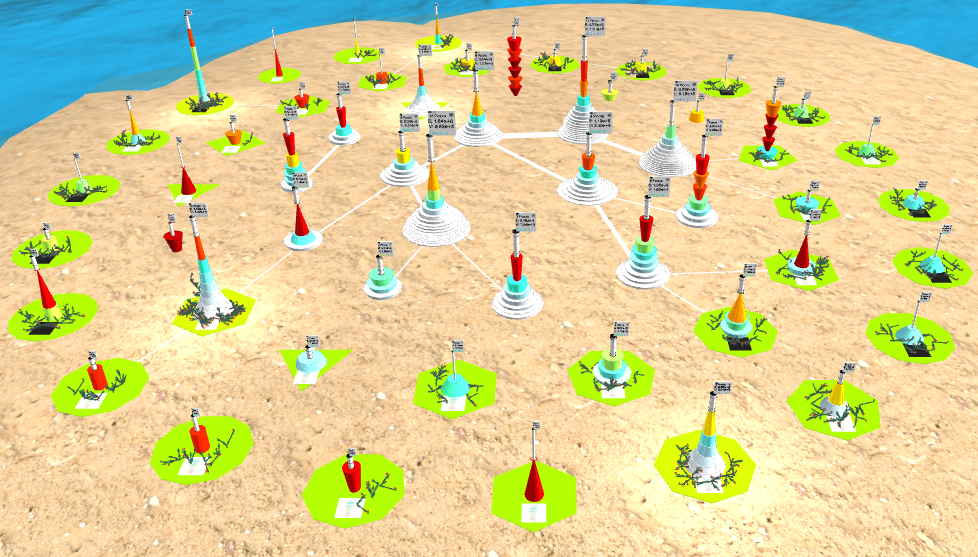
\includegraphics[width=7cm]{imgs/graph_city2.png}
    \caption{Generated Graph City for AML}
    \label{fig:DataFlowDiagram}
\end{figure}
\item We link the Graph City Front-End to our application.
\end{itemize}
}
\textnormal{
The application is used to connect to Graph City and provide a high-level visual representation of the data. The user can now explore the network clusters that can be used to initiate an analysis of the data:}
\begin{itemize}
    \item Explore a cluster in Graph City
    
    \begin{figure}[htp]
    \centering
    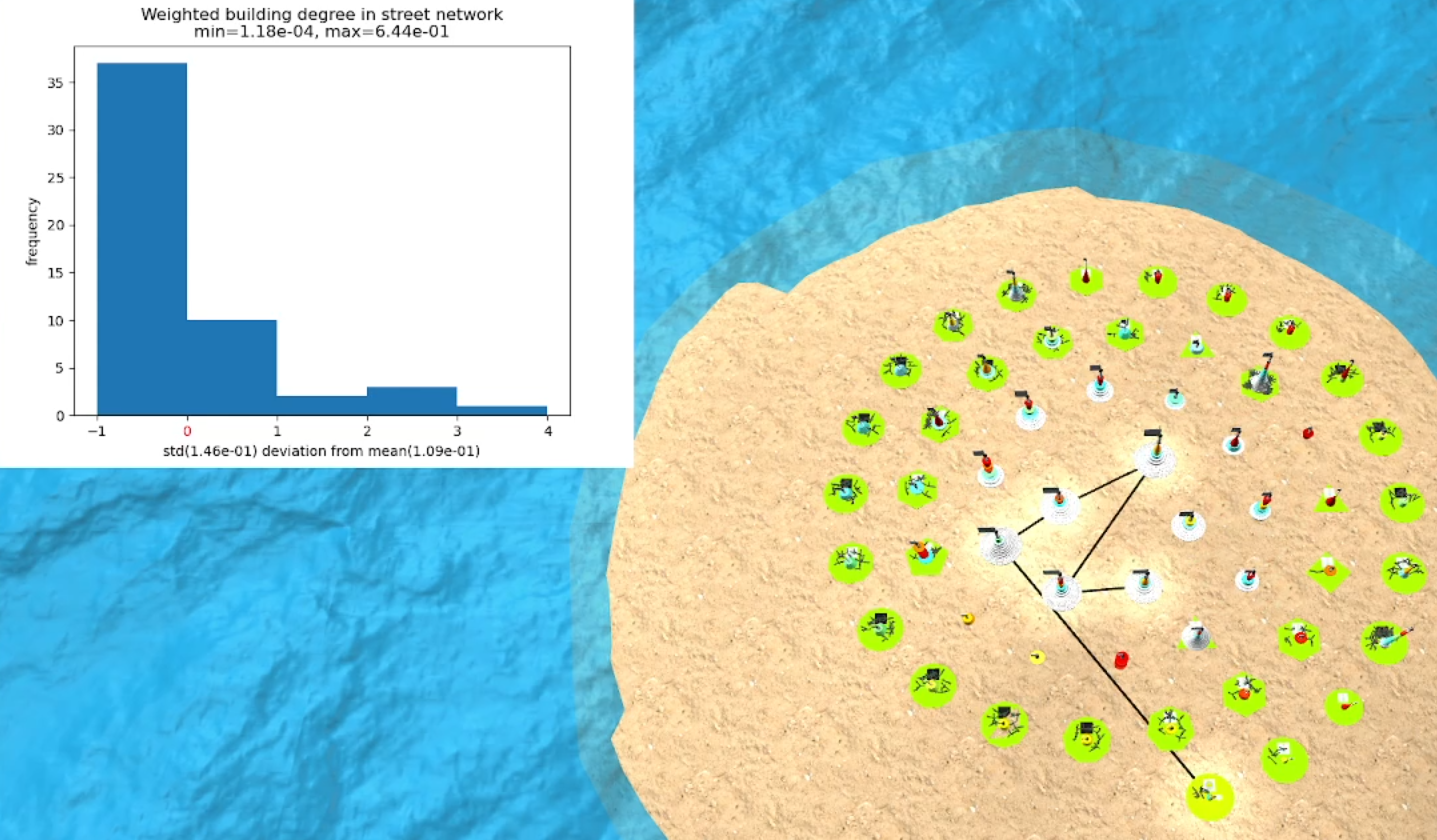
\includegraphics[width=7cm]{imgs/exploration.png}
    \caption{Data Exploration}
    \label{fig:FlowDiagram}
    \end{figure}
    
    \begin{figure}[htp]
    \centering
    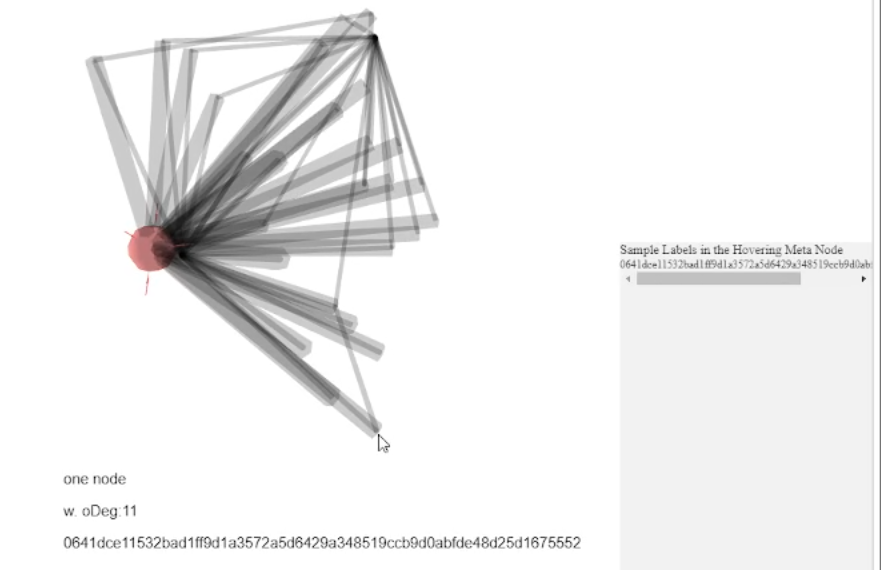
\includegraphics[width=7cm]{imgs/nodeexlore.png}
    \caption{Node Exploration}
    \label{fig:DataFDiagram}
    \end{figure}
    \item Click on a node to redirect to our app to query Neo4j
    \item Generate the cluster visualization of connected nodes
    
    \begin{figure}[htp]
    \centering
    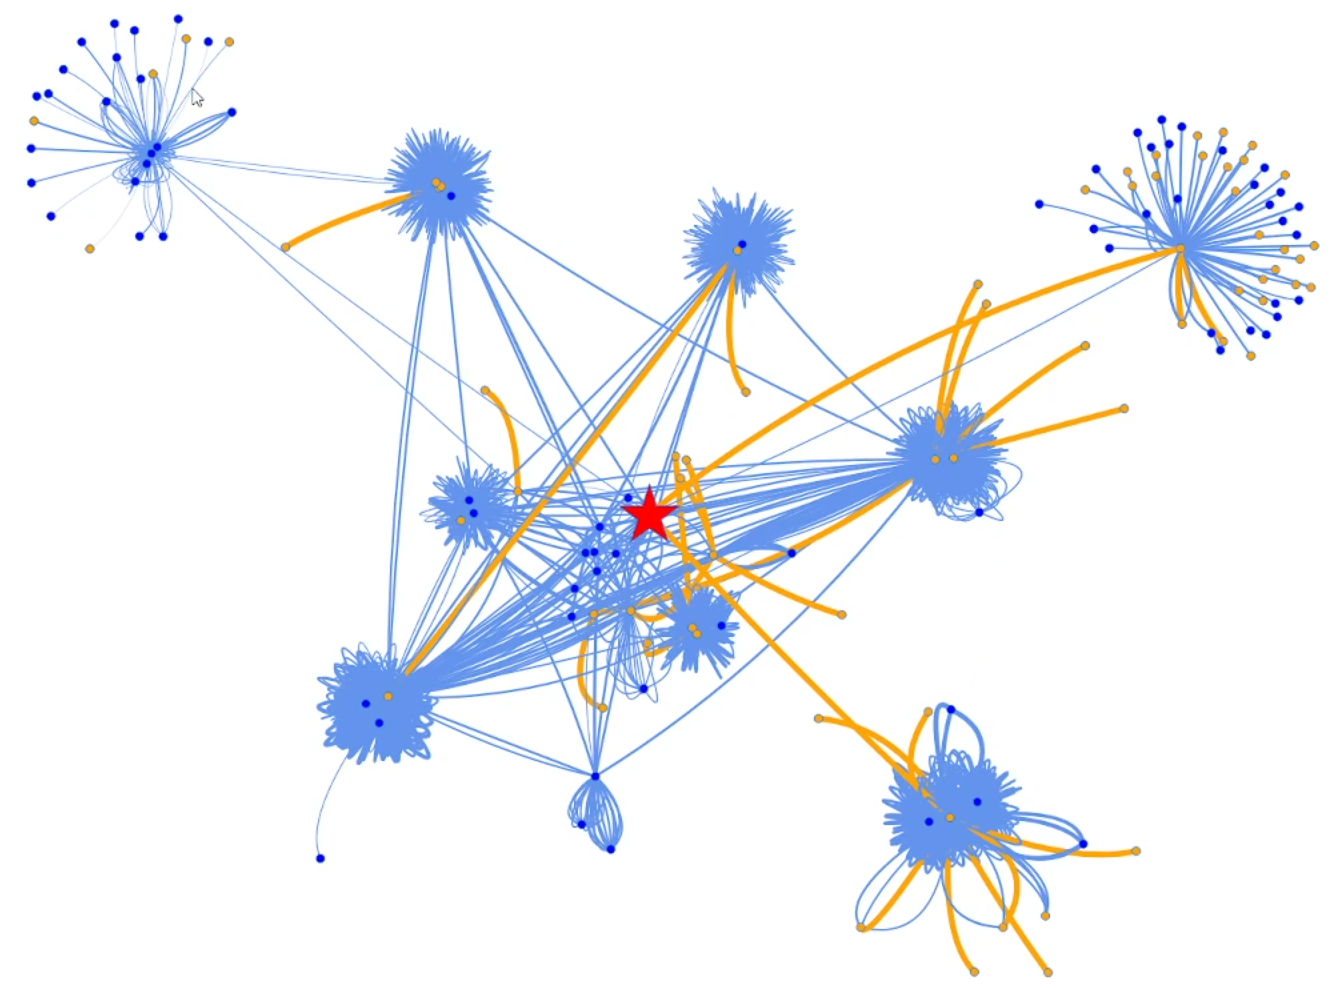
\includegraphics[width=7cm]{imgs/laundering.png}
    \caption{Connected Node Exploration}
    \label{fig:Data}
    \end{figure}
    \item Find laundering transactions and follow laundering chains
    
\end{itemize}